\documentclass[11pt,a4paper]{article}
\usepackage{theme/lmuthesis}

% this for draft water mark
\input{condition}
\ifthenelse{\boolean{release}}{
}{
    \usepackage{draftwatermark}
    \SetWatermarkText{DRAFT}
    \SetWatermarkScale{1}
}

% meta informations
\department{Institut f\"ur Informatik}
\lfe{Lehr- und Forschungseinheit Medieninformatik}
\professor{Prof.\ Dr.\ Andreas Butz}
\type{Master's Thesis}
\title{Explanation Adaptation for Hybrid Multimedia Recommendation System}
\author{AUTHOR}
\email{EMAIL}
\bearbeitungszeitraum{START bis END} 
\supervisor{SUPERVISOR}
\taskdescription{
    \begin{description}
        \item[THESIS TITLE]
        \item[Problem Statement] TO BE ADDED
        \item[Scope of the Thesis] TO BE ADDED
        \item[Tasks] TO BE ADDED
        \item[Requirements] TO BE ADDED
        \item[Keywords] TO BE ADDED
    \end{description}
}
\acknoledgement{
    I would like to appreciate ...
}
\abstract{
    This thesis proposes ...
}

\begin{document}

\makecover
\maketaskdescription
\makededication
\makeabstract
\maketoc
% optional:
% \listoffigures
% \listoftables
\cleardoublepage

\section{Introduction}
\label{ch:intro}

\epigraph{That men do not learn very much from the lessons of history is the most important of all the lessons that history has to teach.}{Aldous Huxley}

\subsection{History of Recommendation System}
Review the changes in the way we look for information so far since the birth of the Internet. In the earliest days, information was scarce. The scattered information led to low efficiency of searching. The main method of information transmission was that people looking for information. Later, the information has gradually been enriched. Some people or companies have gathered kinds of information on some websites, and people can search through the category navigation.
\par With the increasing amount of information, artificially added categories can no longer cover all information, so another type of information acquisition way - search, is born. Typical companies are Google and Baidu.
\par With the development of communication technology and data science, the relationship between people and information has evolved from one-way people looking for information to the current two-way relationship. People find what they need in massive amounts of information, and at the same time, massive amounts of information are also find ways to matching with the audience.
\par Balabanovic designed an adaptive agent for automated web browsing\cite{balabanovic1996adaptive}, in which we can see the prototype of the original recommendation system. Such traditional recommendation systems are unsatisfactory because most of the recommendation systems we use today only make recommendations. Users do not understand the reason and meaning of recommendations. In many cases, if the recommendation algorithm is not accurate or is completely wrong, the results of the recommendation will be strange and deepen the users' doubts and distrust. Recommendations are generated by the entire black-box operations. Users cannot choose but passively accept recommendations and cannot improve the effect of recommendation through interaction.
\par Yongfeng et al. introduced " Explainable Recommendation " which was a new survey and perspectives for recommendation system\cite{zhang2018explainable}. However, much of the research up to now has been descriptive in the generation of explanation. What we can do with explanations and what feedback users can give to the system about the explanation. Based on feedback on explanations, what optimizations can the recommend system make for that and how can it make such optimizations. Little research has been done on these issues.
\par In this paper, we compare the different ways in 5 recommendation styles, provide an overview of the relationship among recommend system, recommendation explanation, and explanation adaptation. We explore the ways in which design an adaptation style for the recommendation explanation module and feedback scoring module. And we propose a new methodology for the "adaptation rule" or "adaptation algorithm" of recommendation explanation.
\par From this evolutionary process, we can see that the emergence of recommendation systems has two important prerequisites, one is information overload, and the other is ambiguous requirements. With the rapid development of today's technology and the increasing amount of data, people feel more and more helpless in the face of massive data. In order to solve the problem of information overload, the computer scientists have proposed a recommendation system, which corresponds to a search engine and can also be referred to as a recommendation engine.
\par Search engines require people to have a clear purpose. They can turn people ?s search for information into precise keywords, then give them to the search engine and finally return them to a series of lists. Users can give feedback on these results. But it will have the problem of the Matthew effect\cite{merton1968matthew}, which will cause the more popular things to become more popular as the search process iterates, making those less popular things sink to the sea.
\par The recommendation engine is more suitable for people who have no clear purpose, or that their purpose is ambiguous. Generally speaking, the user does not even know what he wants. The user's historical behavior or the user's interest preferences or the user's demographic characteristics are transmitted to the recommendation system, and then the recommendation system uses some algorithm to generate a list of items that the user may be interested in. The user is passive to search engines. People only focus on high-exposure items and ignore low-exposure items, which is called the long-tail theory\cite{anderson2004long}, can be used to explain the correctness and rationality of the recommendation system well. Experiments have shown that the low-exposure items in the long tail position generate no less than profit from selling only high-visibility items. The recommendation system can provide opportunities for all items to be recommended, for discovering the potential profits of long-tail projects.
\par When a user's needs are clear, he tends to use search. When the requirements of the user are not clear, some behaviors and preferences data based on the user's history can be used to generate a pre-recommendation, to make the user stay in the system. Some new demands may arise during the user's browsing of information.
\par From the above sections, we can see that the recommendation system is a multi-win-win thing:
\par For users, they can discover what they are interested in and improve the user experience;
\par For items, it is possible to discover the utilization efficiency of long-tail items and revitalize the overall resources;
For the platform, it is able to capture user value and business value.

\subsection{Interaction Between People and Internet}
We can divide the scenarios where people interact with the Internet into three situations as shown in figure \ref{figure:1-1}.

\begin{figure}[h]
\caption{Interaction styles between people and Internet}
\label{figure:1-1}
\centering
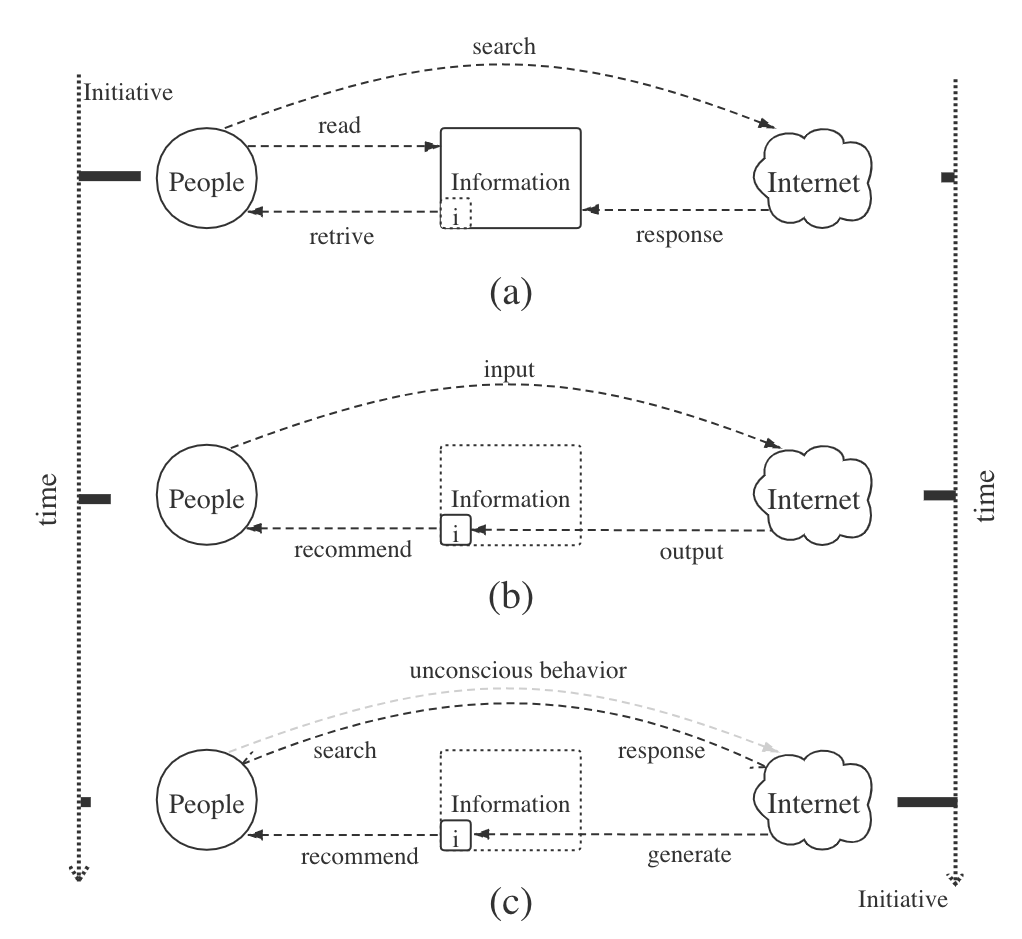
\includegraphics[width=0.8\textwidth]{people_internet_interaction}
\end{figure}

\par \textbf{(a):} People proactive use search engines to get information, and the Internet generates corresponding search results based on what users search for and returns the results according to some organizational structure. The volume of this information "I" is very large and complex. People read this information "I" and try to find the information "i" (i $\in$ I) they need and extract it.
\par \textbf{(b):} People enter some information, and the Internet outputs some recommendations through a recommendation system, and selects a small part of the information that the user needs from a huge information stream, and sends it to the user.
\par \textbf{(c):} The recommendation engine actively searches for audiences that match the content it is recommending, collects data generated by users' unconscious behaviors on the Internet, and analyzes it. In addition, it will actively generate information and recommend that to the corresponding people. For example, a customer purchased a certain product x on Amazon. After a few days, he watched the video on Youtube and found that the advertisement before the video was put by the manufacturer of product x. And the advertising content was about another product y similar to product x. This is one of the ways in which (c) interaction scenarios simply appear in our lives. In the future, human interaction approaches for the recommendation engine based on the scenario (c)  will be more natural and diverse.
\par From a vertical perspective, over time and the development of computer technology. Human initiative is decreasing, and correspondingly, Internet initiative is increasing. This may be the trend of future recommendation system development.
\par Internet giants such as Google and Baidu, which relied on the advantages of search engine technology in the early days, quickly grew into giant companies in the Internet industry. With the development of Internet technology and computing science today, the speed of information generation and transmission is getting faster and faster, and the volume is getting larger and larger. The recommendation system plays a very important and irreplaceable role in the interaction between people and the Internet, as described in (b). But on the other hand, we can see in (c) that recommendation engines have great development potential to achieve the same magnitude as search engines. In this paper, we will do some valuable research and exploration in aspects such as explanation and adaptation for recommend system.

\subsection{Our Contributions}
In this paper, we compare the different ways in 5 recommendation styles, provide an overview of the relationship among recommend system, recommendation explanation, and explanation adaptation. We explore the ways in which design an adaptation style for the recommendation explanation module and feedback scoring module. And we propose a new methodology for the "adaptation rule" or "adaptation algorithm" of recommendation explanation.

\cleardoublepage
\section{Related Work}
\label{ch:related-work}

\epigraph{That men do not learn very much from the lessons of history is the most important of all the lessons that history has to teach.}{Aldous Huxley}

\subsection{Recommend System}

the related-work part 1.
	\subsubsection{conversational RS and Hybrid RS}

\subsection{Explanation Recommend System}

the related-work part 2.

\subsection{Adaptation for ExplanationRecommend System}

the related-work part 3.

\cleardoublepage
\section{System Design}
\label{ch:system-design}

\epigraph{That men do not learn very much from the lessons of history is the most important of all the lessons that history has to teach.}{Aldous Huxley}

\subsection{System Architecture Diagram}
\begin{figure}[h]
\caption{System Architecture}
\centering
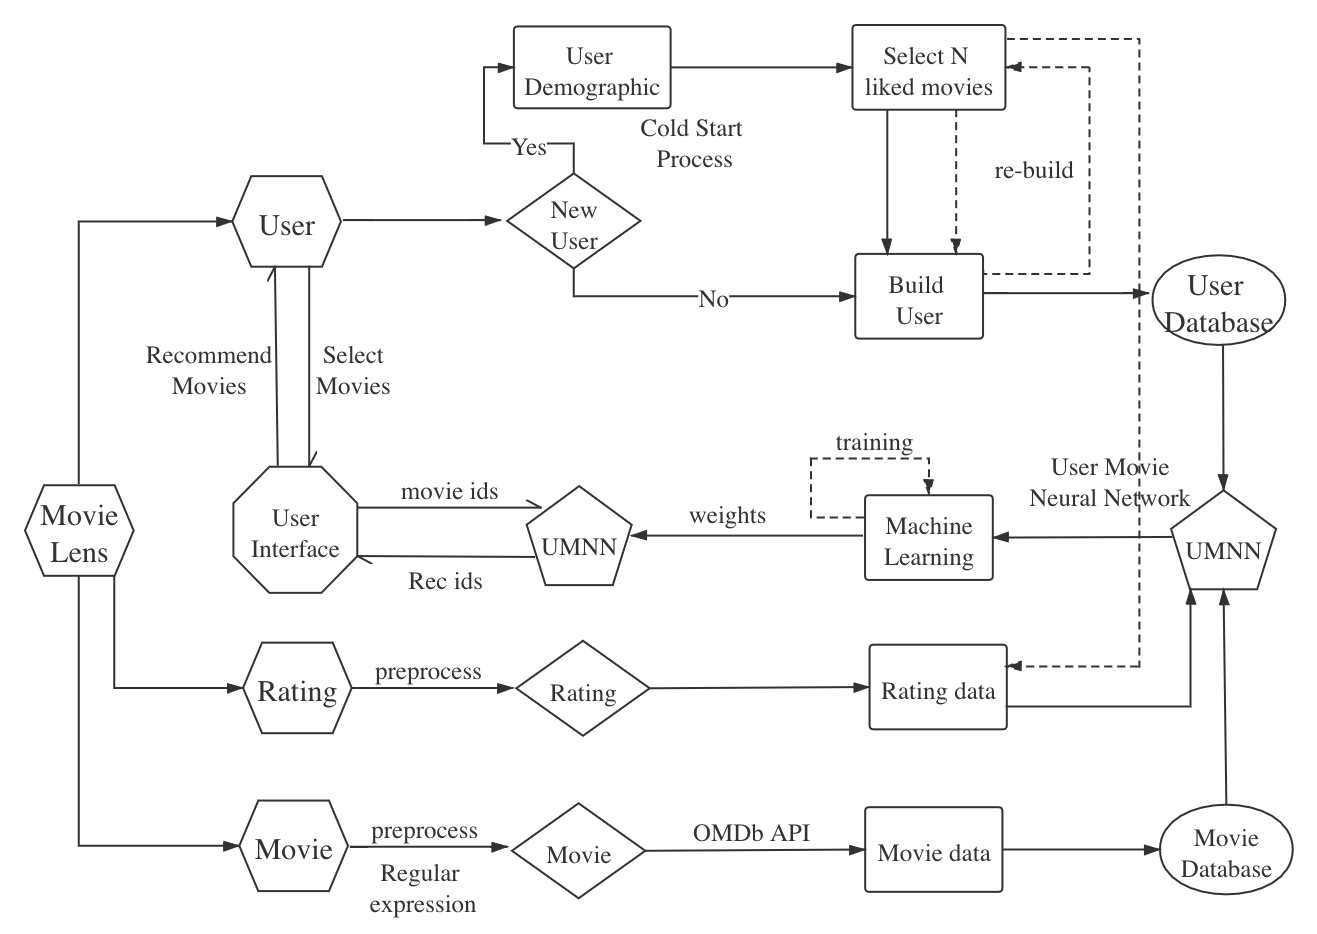
\includegraphics[width=1.0\textwidth]{system_architecture}
\end{figure}
\subsubsection{MovieLens Dataset}
%build user database and movie database
We have selected the MovieLens dataset from the GroupLens Research Group at the University of Minnesota. The MovieLens 1M dataset is used as the data source in this paper. It contains 1 million ratings of 4,000 movies from 6,000 users. It is divided into three tables: movie ratings, movie metadata (genre style and age), and demographic data about users (age, zip code, gender, and occupation).
\subsubsection{UMNN}
\subsubsection{Frontend and Backend}
\subsubsection{Cold Start}

\subsection{Recommendation Strategy}
\subsubsection{Recommendation Style}
\begin{itemize}

\item[(a)]\textbf{Popularity-Based}\\
There are two reasons for recommending based on popularity. First, popularity often represents the important characteristics of a product. Some users utilize extensive sources of information before making decisions to choose a movie, however, the others depend on simple and limited sources of information. But they all will be affected by the popularity of movies to some extent. Second, the popularity of a movie greatly influences user's decisions. From a psychological perspective, when recommending popular movies to users, even if they are not the type the user likes, users usually subconsciously give these movies a higher rating\cite{ahn2006utilizing}. So popularity-based recommendation is a very important and simple method in the early days. In this paper, popularity-based method is used as the basis for the other four recommendation methods.
\item[(b)]\textbf{User-Based}\\
\begin{figure}[h]
\caption{user-based recommendation strategy}
\centering
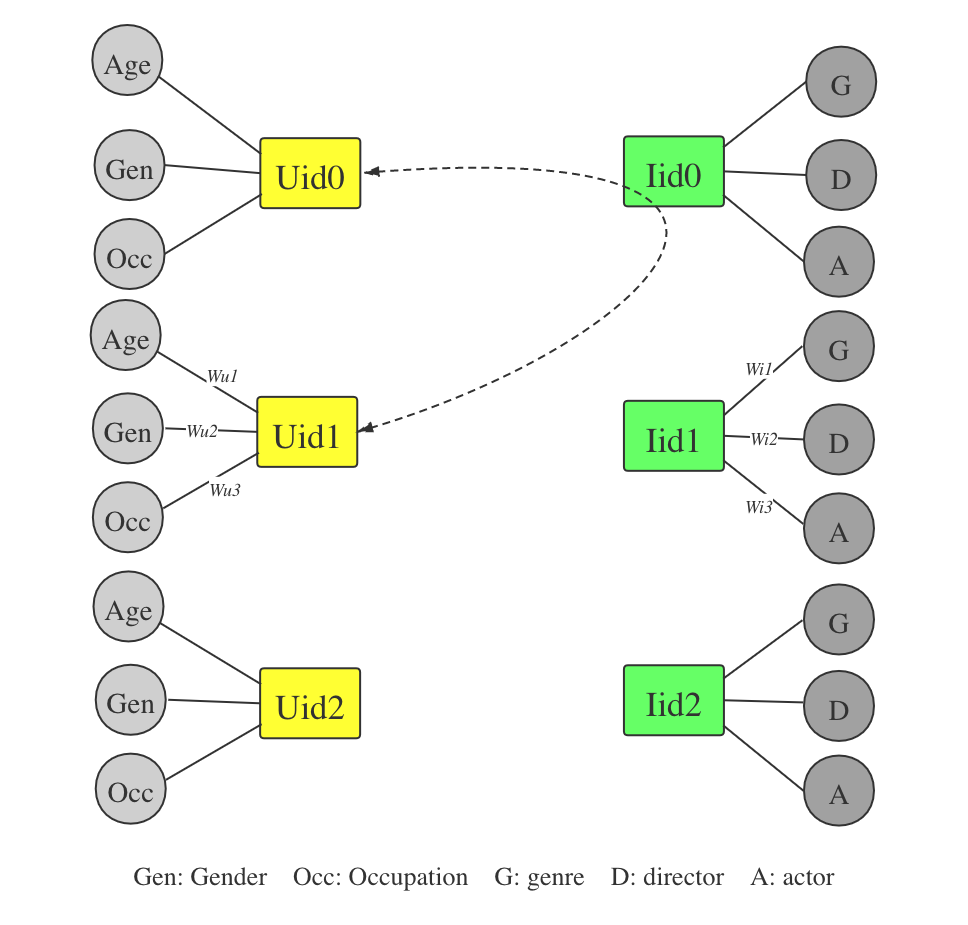
\includegraphics[width=0.5\textwidth]{neural_network_user_based}
\end{figure}
The user-based recommendation strategy more considers the interests of new user and other users with the same hobbies, recommends items that other users like / visited to the new user, and has little to do with new user's current behavior.What will be recommended to a new user, depends on what the other users have visited before. The recommended items are the favorite items of users with the same hobby, so it has a hotspot effect. it can recommend the items that the other users have just visited. It has strong real-time performance, especially the newly introduced hot spots, which can spread quickly and solve the cold start problem of new-item.
\item[(c)]\textbf{Item-Based}\\
\begin{figure}[h]
\caption{item-based recommendation strategy}
\centering
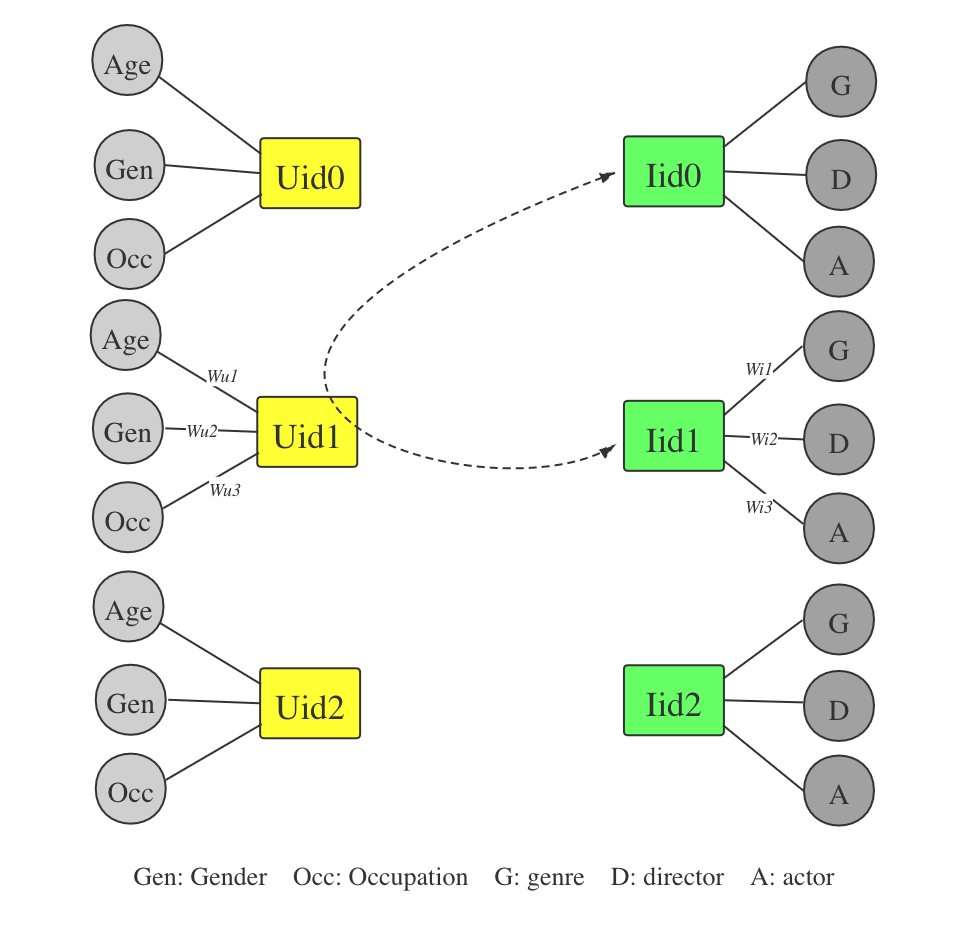
\includegraphics[width=0.5\textwidth]{neural_network_item_based}
\end{figure}
Item-based mainly uses users' historical interests to make recommendations. Recommending items that are similar to the user's history. This method has a lot to do with the user's current behavior. The similarity between the item recommended to the user and the item previously selected by the user is understandable by the user, which is called Interpretable. Most of the recommended items are not popular, but are related to the interests of users. This recommendation method has the highest accuracy when the user's interest is long-term and fixed. The significance of Item-based recommendation is to help users find items related to their interests. The recommended item is not related to user identity, so it is better to solve the problem of new users.
\par Badrul et al.\cite{sarwar2001item} compared the performance of user-based and item-based and demonstrated that the item-based algorithm provides better quality of prediction than the user-based algorithm.
\item[(d)]\textbf{Demographic-Based}\\
\begin{figure}[h]
\caption{demographic-based recommendation strategy}
\centering
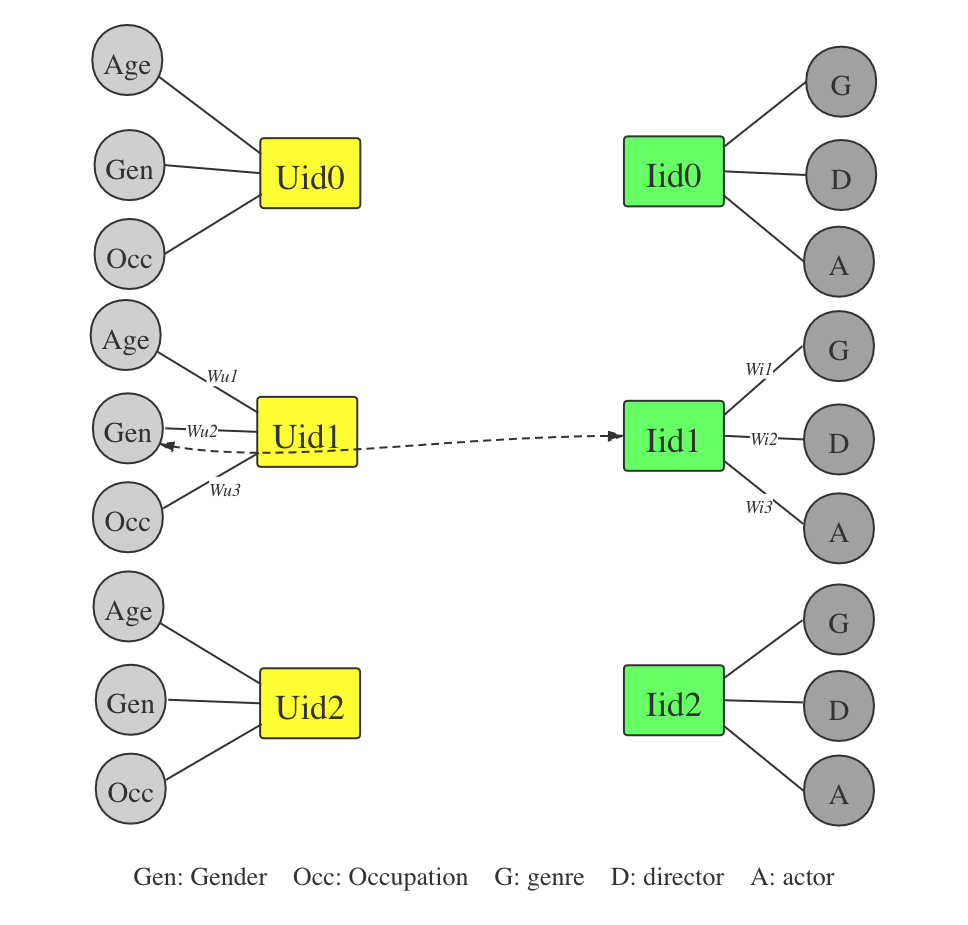
\includegraphics[width=0.5\textwidth]{neural_network_demographic_based}
\end{figure}
According to the basic information of the system user, find out the relevance of the user, and then make recommendations. At present, it is rarely used alone in large systems, and it is usually used in combination with other recommendation algorithms. The usual method is to classify the user based on the user's registration information, and then recommend to the user the items in the category to which she belongs. In this paper, we use gender, age and occupation of user as feature of demographic-based recommendation method.
\item[(e)]\textbf{Content-Based}\\
\begin{figure}[h]
\caption{content-based recommendation strategy}
\centering
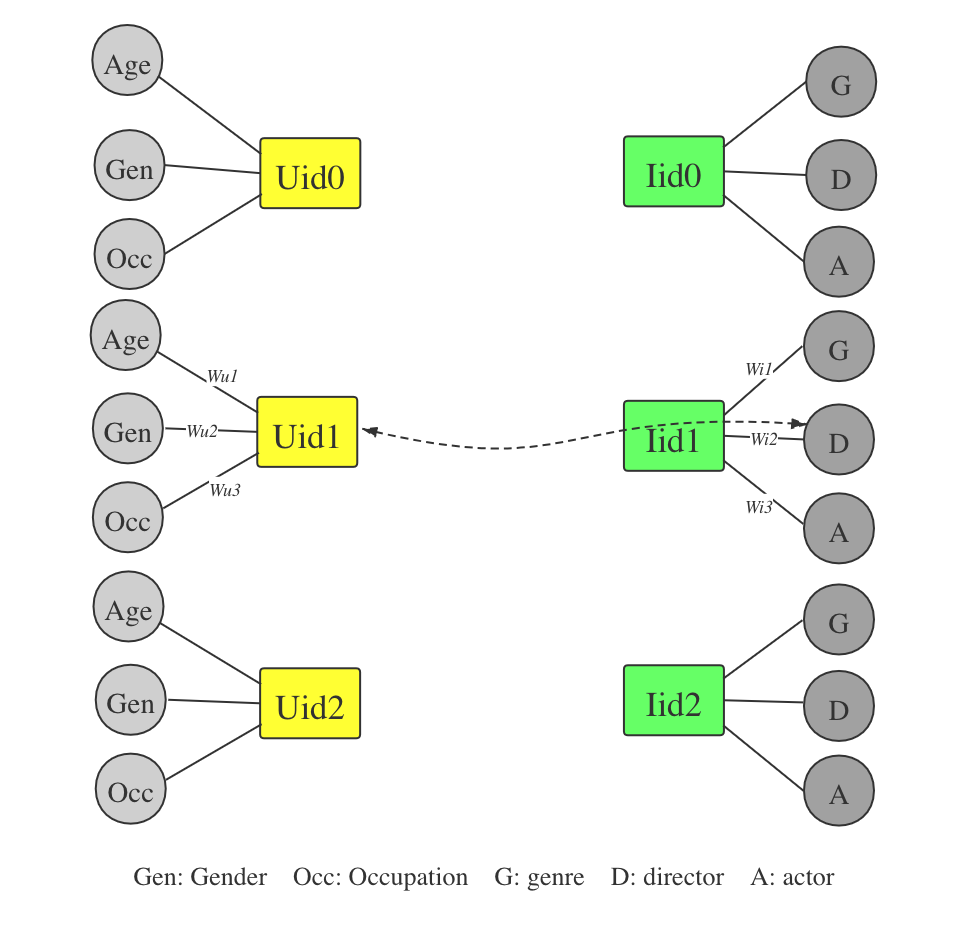
\includegraphics[width=0.5\textwidth]{neural_network_content_based}
\end{figure}
Based on the user's past browsing history, make recommendations to the user that he/she has not viewed. Recommendations are generally based on keywords or content features. For example, if a user has previously chosen to be interested in a certain director's movie, the user will be recommended with the other movie works of this director. The advantage of this method is that there is no popularity bias, items with rare features can be recommended, and user content characteristics can be used to provide recommendation explanations. The disadvantage is that the content must be machine-readable and meaningful, and the features of the recommended content need to be archived in advance.
\par Recommend movies that are similar to movies that users have liked. It is mainly based on the comparison of movie attribute information and user portrait information. The core problem is how to establish the association between movie attributes and user information. it assumes that users will rate items having alike features similarly\cite{safoury2013exploiting}.

\end{itemize}

\par For various reasons, it is easier to collect the user's past behavior than to collect user information, but CF-based (user-based and item-based) has his limitations. When the scoring is very sparse, the prediction accuracy will be greatly reduced. And the cold start of new products is also a problem for CF. In general, therefore, most of today's recommendation systems use a hybrid recommendation method.
\subsubsection{Recommendation Explanation Strategy}
\subsubsection{Recommendation Explanation Adaptation Strategy}
%rule based

\subsection{Machine Learning Algorithm}

\subsubsection{Tool and Library}
%weights
PyTorch\cite{ketkar2017introduction} and TensorFlow\cite{abadi2016tensorflow} are currently the most popular methods for investigating deep learning and neural networks. PyTorch is more useful for researchers, enthusiasts and Individual developers to quickly build prototype in small-scale projects. TensorFlow is more suitable for large-scale deployments, especially when cross-platform and embedded deployments are required. In our research, PyTorch was selected for its vast repository of libraries to handle dataset preprocessing, statistical analysis, plotting, and more.\cite{paszke2019pytorch}.

\subsubsection{Neural Network Model}
%node and item
\subsubsection{Training Weights}


\subsection{User Interface Prototype} 

\subsubsection{Development Tool and Language}
\subsubsection{Prototype}
\subsubsection{}

\subsection{}

\cleardoublepage

\section{Experiment}
\label{ch:experiment}

\epigraph{That men do not learn very much from the lessons of history is the most important of all the lessons that history has to teach.}{Aldous Huxley}

\subsection{User Study Process}
Let users use our recommendation system, record their feedback and answers to the questionnaires, and analyze data to evaluate the performance and interpretability of our recommendation system.
\par After reading the explanations about the user study, users will input some personal data (user id, gender, age and occupation) and then answer some background questions. For building user Pprtraits, system will give user a series of movie posters and names. user can click to select the movies he likes from 6 options. Click the ?REFRESH? button to load the new 6 options and repeat this selection process until the user has selected a total of 10 movies. After that, the system will give user a series of recommendation movies and the explanations why these are recommended to the user. The user can click to select the movies he likes and give a score for the explanations. Repeat this recommendation step three times. Finally, the user will be required to answer some feedback questions.

\subsection{likert Scale}
The statistics of the questionnaire about system evaluation by using likert scale are shown in figure \ref{figure:1}.

\begin{figure}[h]
\caption{Feedback question about system evaluation}
\label{figure:1}
\centering
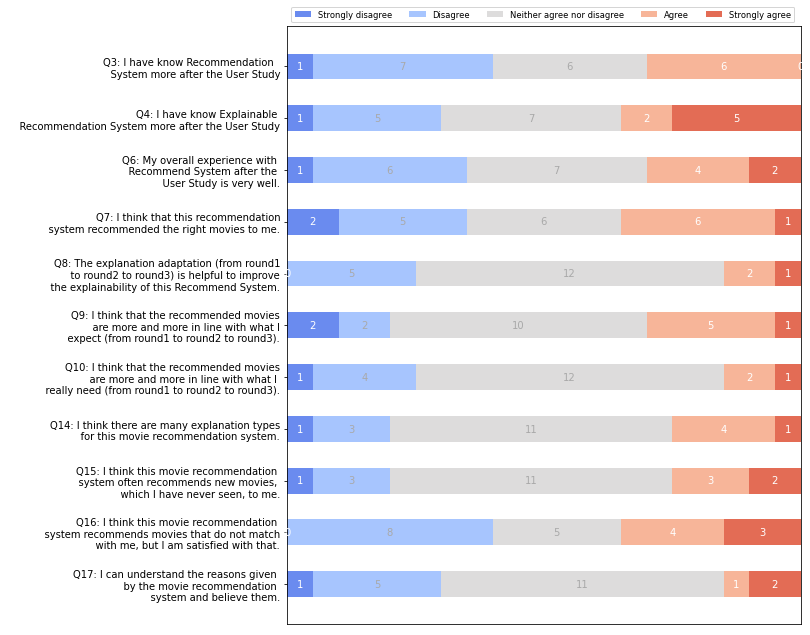
\includegraphics[width=1\textwidth]{feedback_question3}
\end{figure}

Figure \ref{figure:2} presents the results obtained from the preliminary analysis of points for 3 round recommendations from 20 users. We can see that the third round reported more high-points than the other two rounds. This shows that in our user study, the average score of users improved through three rounds of explanation adaptation.

\begin{figure}[h]
\caption{Feedback question about 3 round recommendations}
\label{figure:2}
\centering
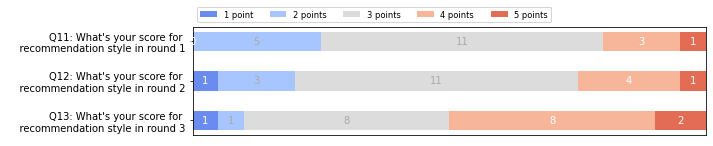
\includegraphics[width=1\textwidth]{feedback_question2}
\end{figure}



\subsection{User Study Metric}
Correspondingly, the division of questions for evaluating the recommendation system is shown in the table \ref{table:1}.

\begin{table}[h!]
\renewcommand\arraystretch{1.5}
\centering
\begin{tabular}{p{100pt}p{60pt}p{200pt}}\toprule
 \hline
 System Evaluation & Question & Result \\ [0.5ex] 
 \hline
  Satisfaction & Q8 & More than half of users choose a neutral attitude (12 in 20)  \\
   \cdashline{1-3}[0.8pt/2pt]
    & Q7 & 7 users agree that the system recommend the right movies.\\
  Accuracy  & Q9 & 6 users agree that the system has recommended what they expect. \\
    & Q10 & 3 users agree that the system has recommended what they really need. \\
    \cdashline{1-3}[0.8pt/2pt]
  Diversity & Q14 & 5 users agree \\
  Novelty & Q15 & 5 users agree \\
  Surprise & Q16 & 7 users agree \\
  Trust & Q17 & 3 users agree \\
  [1ex] 
 \hline
\end{tabular}
\caption{Questions for system evaluation}
\label{table:1}
\end{table}

\paragraph{Confidence:}
\paragraph{Transparency:}
\paragraph{Satisfaction:}
\paragraph{Accuracy:}
Comparing the three questions about accuracy ( Q7, Q9, Q10), we can find a very interesting phenomenon. Some users said that the recommendation system recommended the right movies to them, but they thought that the recommendation system did not recommend the movies they really expected and needed.
\par As Abraham argues in \cite{maslow1943theory} about Maslow's hierarchy of needs, from low to high, human needs are divided into physiological needs, safety needs, social needs, esteem and self-actualization needs.
\par Most recommendation systems, including our recommendation system, often recommend things that users may be interested in based on some data and records. This is certainly the right recommendation, but sometimes it may not be what users really expect and demand. The recommended things only satisfy the user's physiological needs, safety needs, and social needs. And higher-level esteem and self-actualization needs may become one of the possible development directions of future recommendation systems research area.
	
\subsection{Result analysis}

\cleardoublepage

\section{Evaluation}
\label{ch:evaluation}


\begin{figure}[h]
\caption{User behavior data}
\label{figure:5-1}
\centering
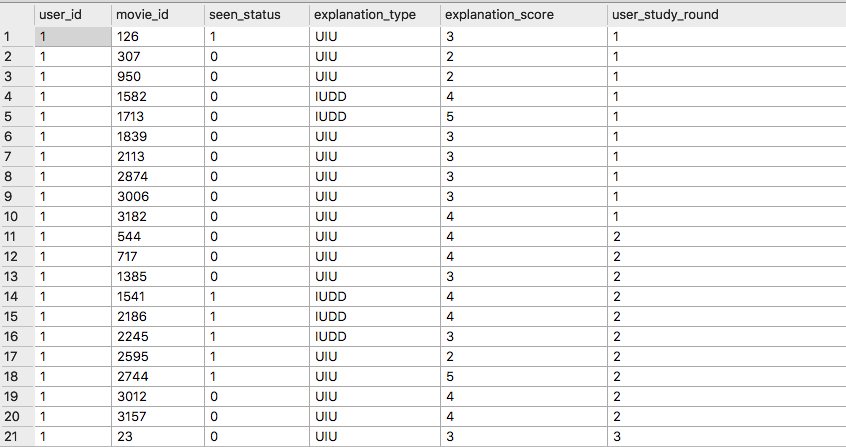
\includegraphics[width=1\textwidth]{database}
\end{figure}

Figure \ref{figure:5-1} is the structure of user behavior data. We collect:
\par the data of users' id
\par All the movies' id that selected by some users
\par Seen status (0:not seen, 1: seen)
\par Explanation type
\par Explanation score
\par Recommendation round number
\par We have already evaluated the data and have used it to build the Likert scale in the user study section.

\cleardoublepage

\section{Application}
\label{ch:application}

\epigraph{That men do not learn very much from the lessons of history is the most important of all the lessons that history has to teach.}{Aldous Huxley}



\cleardoublepage

\section{Discussion}
\label{ch:discussion}

\epigraph{That men do not learn very much from the lessons of history is the most important of all the lessons that history has to teach.}{Aldous Huxley}

\cleardoublepage

\section{Conclusion}
\label{ch:conclusion}

\epigraph{That men do not learn very much from the lessons of history is the most important of all the lessons that history has to teach.}{Aldous Huxley}

% Future research: And higher-level esteem and self-actualization needs may become one of the possible development directions of future recommendation systems research area.
% emotion affective recommendation

\cleardoublepage

\section{Appendix}
\label{ch:appendix}

\epigraph{That men do not learn very much from the lessons of history is the most important of all the lessons that history has to teach.}{Aldous Huxley}

\cleardoublepage


\part*{Bibliography}
\addcontentsline{toc}{part}{Bibliography}
\nocite{*}
\bibliographystyle{apalike}
\bibliography{literatures/list}

\end{document}